\noindent{\bf Dataset Description.} 
%
The data used in this work corresponds to events from August 2013 to June 2015.
%
This dataset consisted of 20,066 news events, which contained 193,445,734 tweets
produced by 26,127,624 different users.

We note that our event representation and applications are independent of the
data extraction methodology.  
%
Therefore, in order to improve the representativeness of our event collection in
the future, less biased methods of event extraction can be used, such as
automatic event detection techniques~\cite{Metzler_2012, Choi_2012} and/or the
integration of more comprehensive sets of seed news sources, as done for Chilean
news analysis by Maldonado et al.~\cite{maldonado2015spatio}.


\section{Exploratory Analysis}\label{sec:geo:mining}
% Implementation

We present an exploratory data mining analysis that uses the information
provided by our spatio-temporal context-aware event representation.  
%
We describe our empirical findings, which illustrate the usefulness of our
proposed event representation.  
%
This analysis considers the location context of events at the country-level
geopolitical division.  
%
This allows us to explore the international interactions given by our current
dataset. 


The event extraction process, described in Chapter~\ref{chapter:data}, was based
on a seed set of internationally renowned news media accounts that publish
information in English. 
%
This introduced a certain bias in our event collection towards events that took
place in English speaking countries, and towards including more tweets in
English than in other languages. 
%
For example, for the event {\it ``correspondents dinner''} our current method
will mostly retrieve tweets in English from users world-wide. 
%
On the other hand, an event described with a set of keywords which includes {\it
``Barack Obama''} will retrieve tweets in several languages. 

%%

These biases must be taken into consideration because they can limit the
representativeness of the findings yielded by our data mining analysis.
%
Nevertheless, we believe that they do not invalidate our results, which show the
perspective of a subset of the social network that is centered on news reported
in the United States and Great Britain. 
%
Therefore, our results reflect the world-view of these two overly represented
countries in particular, and of English-speaking users in general.
%
Furthermore, other studies using the full Twitter stream, such as that of
Poblete et al.~\cite{Poblete:2011:BTS:2063576.2063724}, show a similar data
distribution to ours, indicating that this type of bias could be inherent to
Twitter itself.

%%

Furthermore, an in-depth exploration of the bias in our dataset showed that the
number of tweets produced during an event did not depend on the number of seed
accounts that covered that event. 
%
Our analysis showed that only $13.5\%$ of the users in the entire collection had
actually re-posted a tweet from the seed news media accounts, which gives the
overall impression that these accounts did not influence much the amount of
interest expressed by users. 
%
Also, we found no relation between the number of seed accounts that shared an event
and the number of countries that participated in the event in terms of
provenance or of impact. 
%
(We found no correlation between the proportion of different news
outlets and the number of different users, the protagonist countries, or the
number of tweets from each interested country.)

%%

As mentioned in Section~\ref{sec:relations} we used a normalization for vectors
$\mathbf{pi}$ and $\mathbf{cp}$, defined in Equations~\ref{eq:pi}, \ref{eq:pi-w}
and \ref{eq:cp}, \ref{eq:cp-w}, respectively. 
%
This normalization allows us to compare protagonist-interest and co-protagonist
vectors in a way that mitigates the bias of over-represented countries. 
%
In particular, for the $\mathbf{pi}$ vector we defined $w(l_j,l_k)$ as:

$$w(l_j, l_k) = f(x_{j,k})= \frac{x_{j,k} - \mu(\mathbf{x}_{\cdot,k})}{\sigma(\mathbf{x}_{\cdot,k})}$$

\noindent and for $\mathbf{cp}$ we defined $w'(l_j,l_k)$ as:

$$w'(l_j, l_k) = f(x'_{j,k})= \frac{x'_{j,k}}{x'_{j}},$$

\noindent where $x_{j,k}$ was the number of events that have $l_j$ as
protagonist in which $l_k$ is interested; $\mathbf{x}_{\cdot,k}$ is the vector
containing the number of events in which location $l_k$ is interested, $\forall
l_j \in L$; $\mu$ and $\sigma$ are the mean and standard deviation of the
distribution of events, respectively; $x'_{j,k}$ is the number of events for
which both $l_j$ and $l_k$ were protagonists, and $x'_{j}$ is the number of
events that had $l_j$ as protagonist.

% These normalizations
%are optional and not part of our model, as they are not always used by
%the application, such as the case of our visualization tool presented
%in Section~\ref{sec:vis}.
\begin{figure*}[t]
\centering
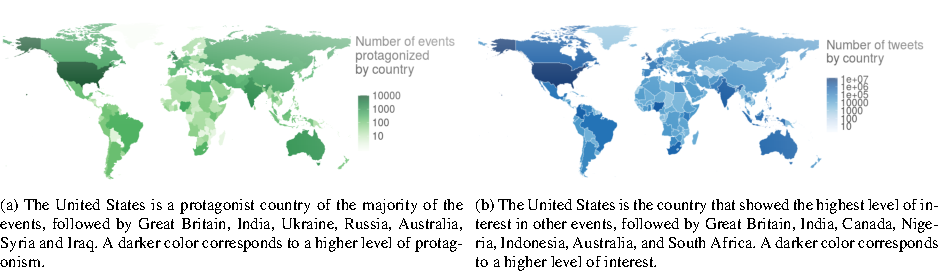
\includegraphics[width=\textwidth]{figures/geopolitical/choropleths.pdf}
\caption{Summary maps of interest and protagonists.}\label{fig:maps}
\end{figure*}

\begin{figure*}[t]
\centering
\makebox[\textwidth][c]{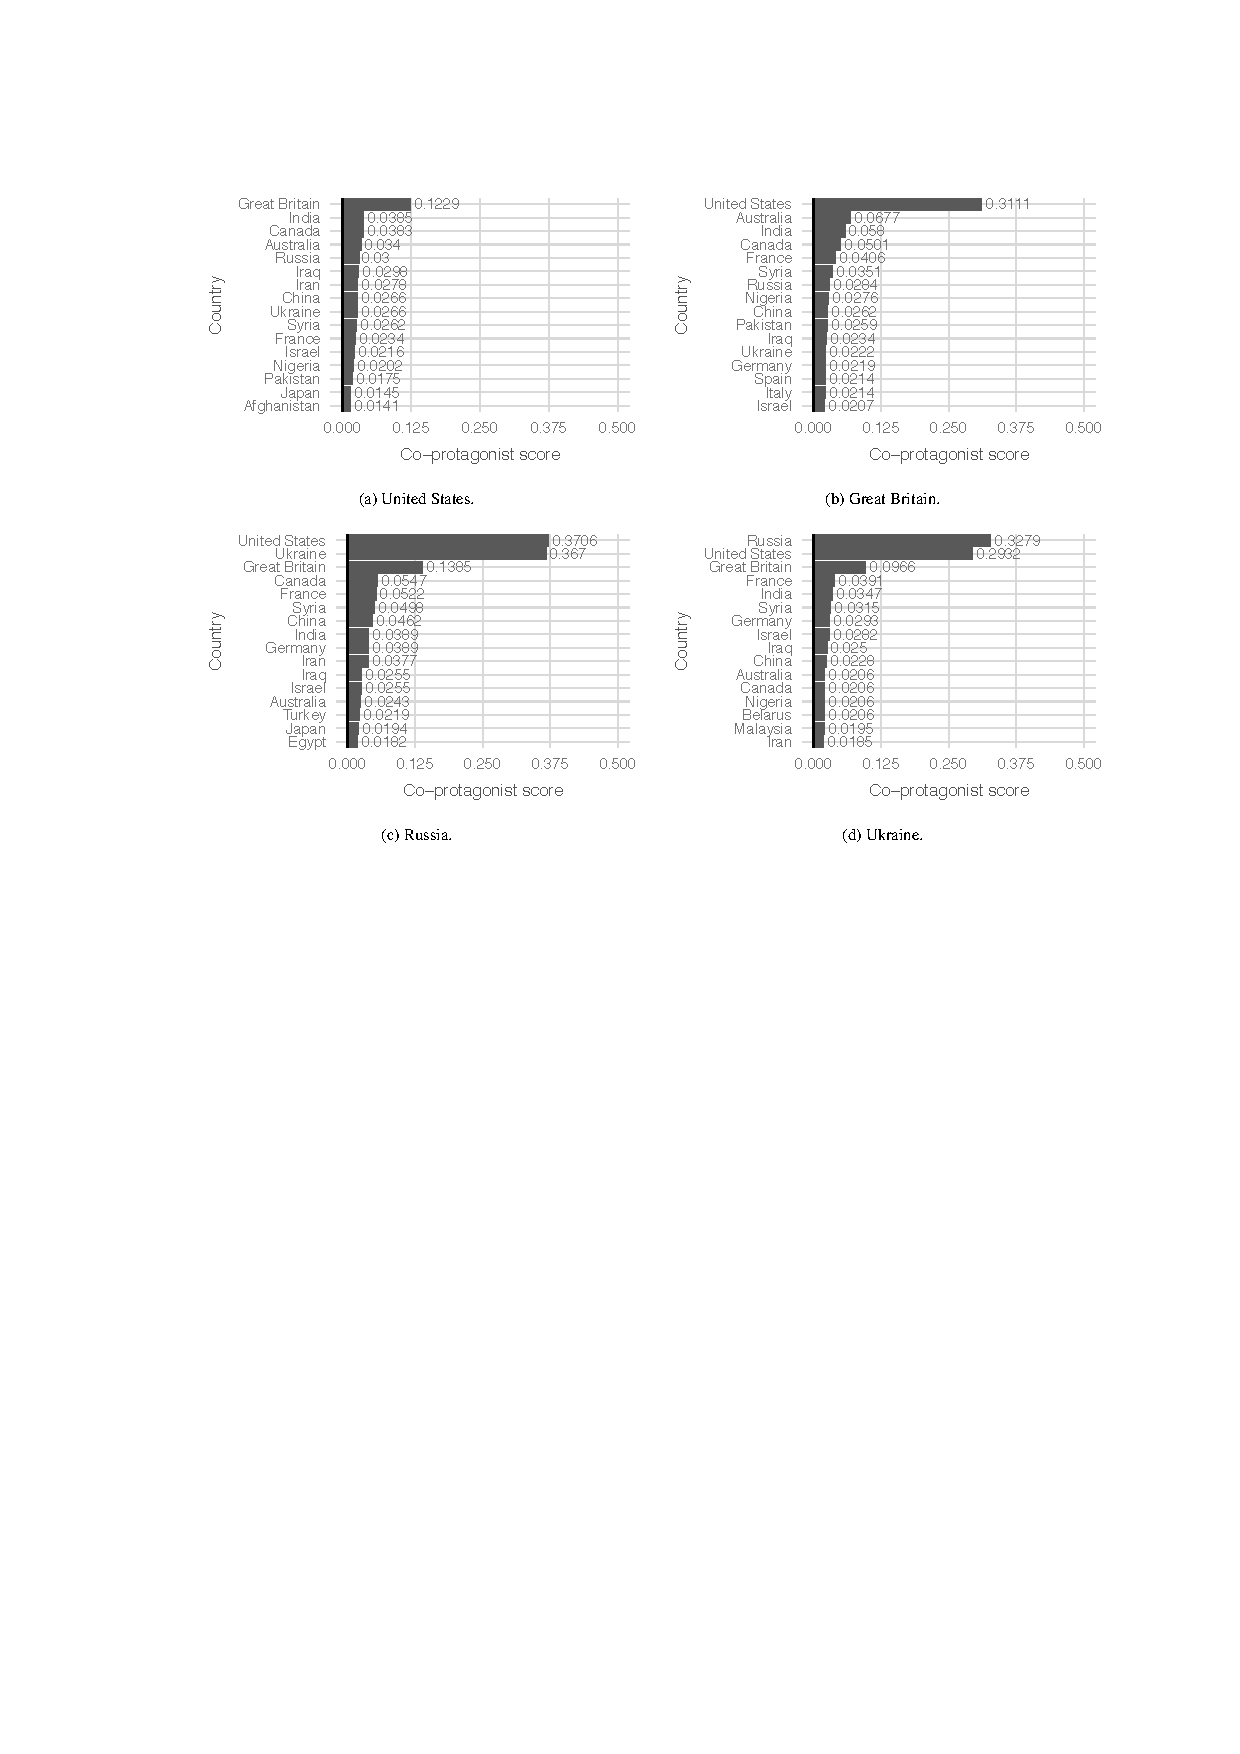
\includegraphics[width=1.1\textwidth]{figures/geopolitical/coprot.pdf}}%
%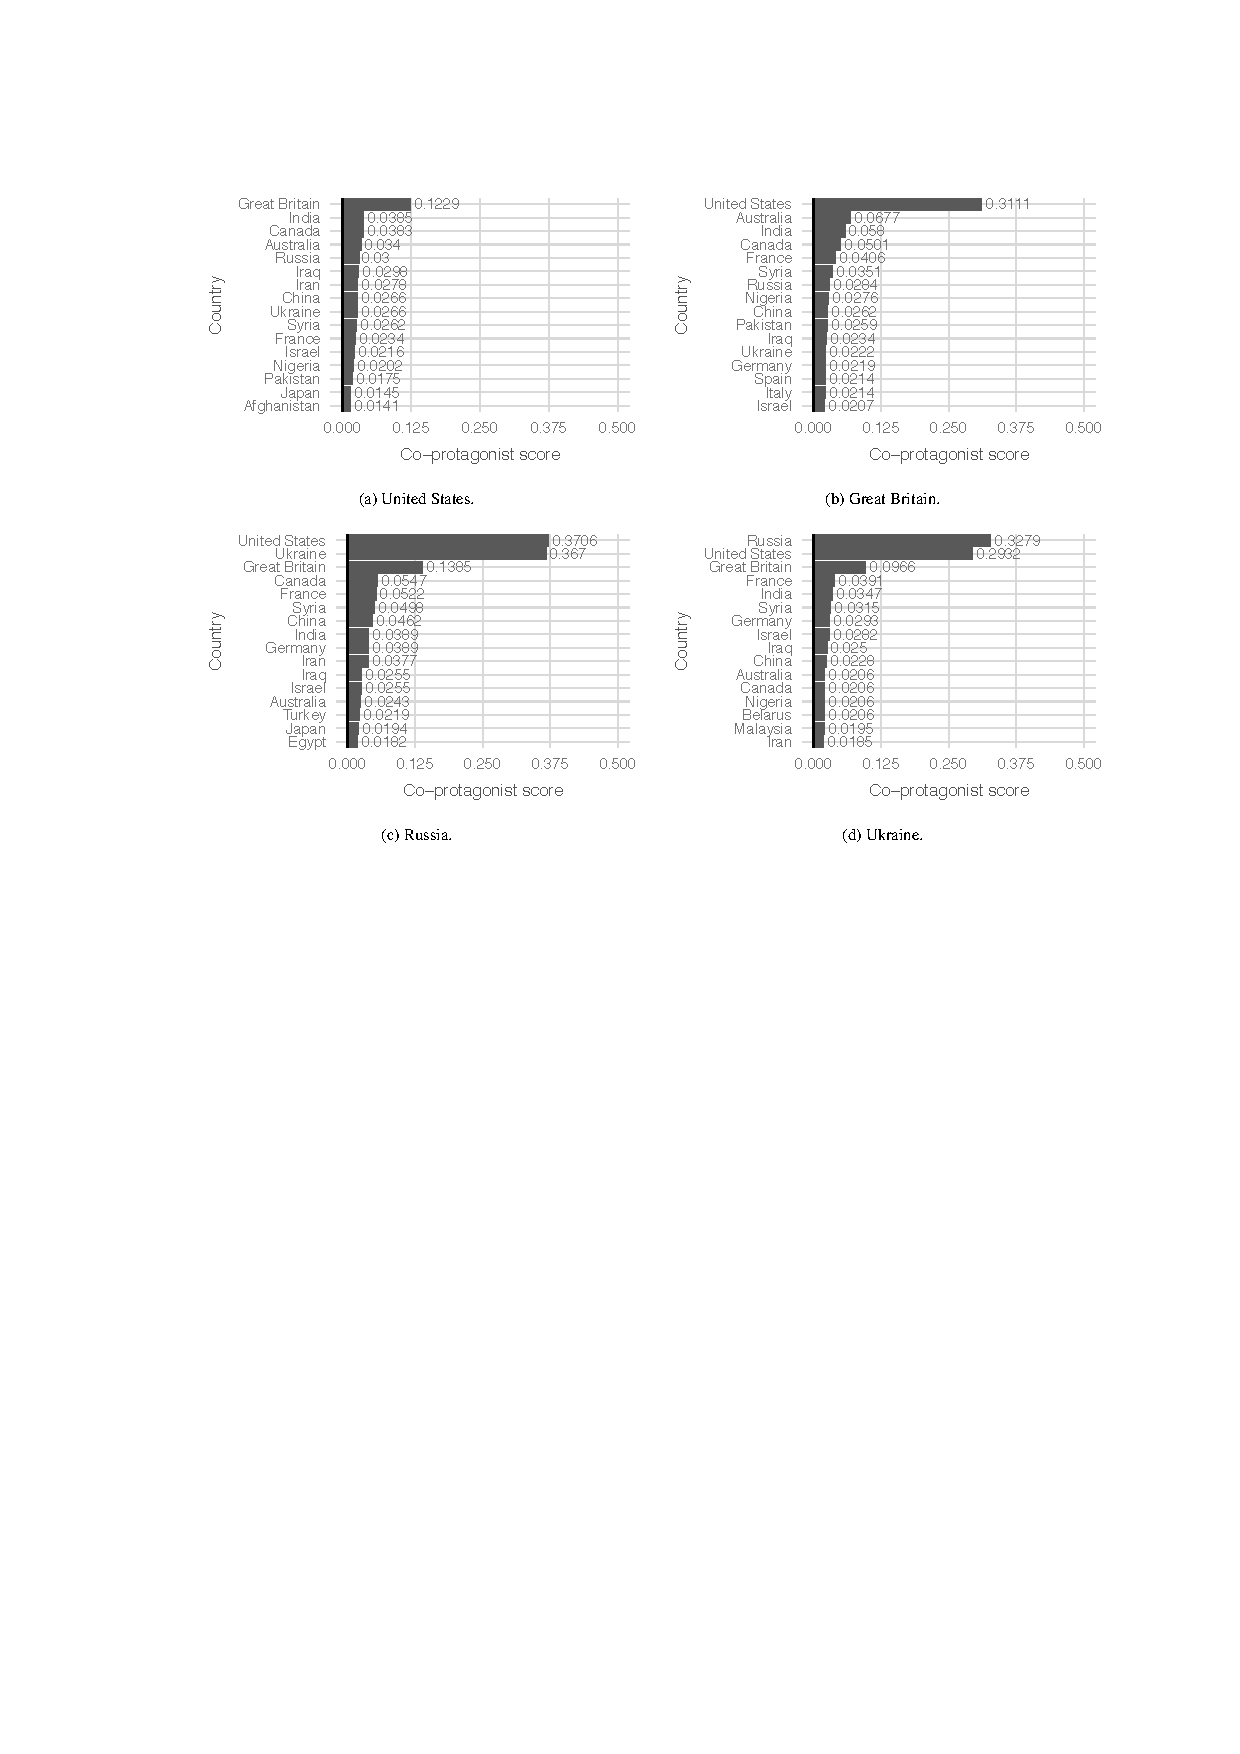
\includegraphics[width=1.1\textwidth]{figures/geopolitical/coprot.pdf}
\caption{Relative co-protagonist measure of selected countries.}\label{fig:coprotagonism-ind}
\end{figure*}

% tweets & users per country
\begin{figure*}[t]
\centering
\makebox[\textwidth][c]{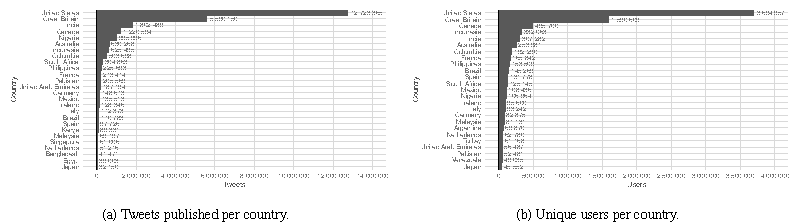
\includegraphics[width=1.15\textwidth]{figures/geopolitical/tweets-users.pdf}}%
%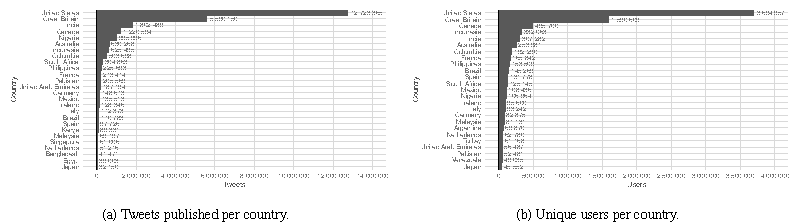
\includegraphics[width=1.1\textwidth]{figures/geopolitical/tweets-users.pdf}
\caption{Description of the bias in the number of tweets and users, per country.}\label{fig:tweets-per}
\end{figure*}



We started by characterizing the spatial distribution of our collection to
describe its representativeness in terms of geographical coverage. 
%
In terms of protagonist locations, the United States and Great Britain were the
protagonists of the majority of the events, followed by India, Australia,
Ukraine and Russia (Figure~\ref{fig:maps} (a)). 
%
The median number of events in which countries were protagonist is $18.5$,
indicating that only a few countries were the protagonists of the majority of
events. 
%
Figure~\ref{fig:maps} (a) shows the distribution of the number of events in
which countries were protagonists. 
%
When we computed the $\mathbf{cp}(c_i)$ vectors for selected $c_i$ countries
(Equation~\ref{eq:cp}, normalized by the number of events in which a country
$c_i$ is protagonist), we observed that the United States and Great Britain were
the protagonists of the majority of international events
(Figure~\ref{fig:coprotagonism-ind}). 
%
There are some exceptions, such as Ukraine, which had only Russia as the
co-protagonist of many of its international events
(Figure~\ref{fig:coprotagonism-ind} (d)).
%There are some exceptions, such as Ukraine which co-protagonizes most of its events
%with Russia (Figure~\ref{fig:co-prot-ua}).

%%

In terms of worldwide interest, the countries that displayed interest in most
events were the United States, Great Britain and India (Figure~\ref{fig:maps}
(b)).  
%
In addition, these countries also contributed the most tweets
(Figure~\ref{fig:tweets-per} (a)).

We determined the location for 37.3\% of the users (9,738,538 out of 26,127,625
users). 
%
These users were mostly distributed among the United States and Great Britain,
followed by Canada, Indonesia and India (Figure~\ref{fig:tweets-per} (b)).
%% \bp{should
%% we say that it is reasonable to expect the geolocated users to be
%% sampled randomly among locations?}

\medskip
\noindent{\bf International relations exploration.}
We explored the dataset in order to identify similarity between countries
according to the events in which they are co-protagonists and the interest shown
towards these events by the rest of the countries in the world. 
%
We found that applying standard similarity metrics over the data in the event
representations, yielded relationships between certain countries that resemble
intense historical interactions and/or geographical proximity.

%\noindent \textbf{Country co-protagonism.}
In terms of protagonist locations, we found countries that were {\em similar},
meaning that they were protagonists of the same events. 
%
In this case we used the Jaccard similarity between each pair of countries as
our similarity measure, representing each country by the set of events in which
it was a protagonist. 
%
The Jaccard similarity between two sets $x$ and $y$ is defined as $sim_{x, y} =
\frac{|x \cap y|}{|x \cup y|}$.
%
We filtered out the countries that were protagonists of fewer than $130$ events
(corresponding to the 80-th percentile of events for which countries were
protagonist). \\

%
\paragraph{Significance of the Jaccard metric.}
%
We studied the distribution of our similarity metric, in order to determine
which relationships between countries were significant. 
%
We fitted the \emph{similarity} to a theoretical probability distribution using
the R package {\em
fitdistrplus}~\footnote{\url{https://CRAN.R-project.org/package=fitdistrplus}}
and we found that the best fit was a Gamma distribution with parameters
$shape=0.8721$ and $rate=85.7683$.
%
Based on this analysis, if $S$ is a random variable with a Gamma distribution
representing the similarities between countries, then we defined the similarity
between two countries $x$ and $y$ as being {\em significant} if its value was in
the 95-th percentile of the distribution, (i.e., if $P( S < sim_{x,y} ) >
0.95$).
%
Using this criteria, we determined a similarity threshold of $sim^*=0.032$,
above which we considered its value to be significant. 
%
This threshold can be parameterized at the 80-th, 90-th, or 99-th percentile, as
the researcher finds appropriate.  
%
Table \ref{tab:jacc} shows the top-20 most similar countries based on this
similarity, making it to the 97.181 percentile of our dataset. \\

\begin{table}
  \centering
  \footnotesize
\begin{tabular}{llrrrr}
\toprule
Country $i$ & Country $j$ & $x'_i$ & $x'_j$ & Similarity & Percentile\\
\midrule
Israel & Palestine & 561 & 360 & 0.2863 & 99.969\\
Russia & Ukraine & 823 & 921 & 0.2094 & 99.906\\
North Korea & South Korea & 158 & 179 & 0.1866 & 99.843 \\
Great Britain & United States & 4,015 & 10,162 & 0.0966 & 99.248\\
Iraq & Syria & 654 & 647 & 0.0833 & 99.092\\
\addlinespace
India & Pakistan & 1,561 & 453 & 0.0753 & 98.998\\
Iran & Israel & 496 & 561 & 0.0698 & 98.841\\
China & Japan & 646 & 354 & 0.0605 & 98.340\\
France & Germany & 627 & 371 & 0.0583 & 98.184\\
\addlinespace
Argentina & Brazil & 130 & 236 & 0.0578 & 98.152\\
Australia & Great Britain & 974 & 4,015 & 0.0577 & 98.090\\
Brazil & Germany & 236 & 371 & 0.0575 & 98.058\\
Syria & Turkey & 647 & 198 & 0.0536 & 97.964\\
\addlinespace
Iran & Iraq & 496 & 654 & 0.0512 & 97.777\\
Australia & Malaysia & 974 & 262 & 0.0492 & 97.682\\
Argentina & Germany & 130 & 371 & 0.0481 & 97.620\\
Australia & India & 974 & 1,561 & 0.0475 & 97.495\\
\addlinespace
Germany & Greece & 371 & 155 & 0.0457 & 97.401\\
Canada & Great Britain & 715 & 4,015 & 0.0444 & 97.275\\
Egypt & Libya & 316 & 253 & 0.0440 & 97.213\\
Great Britain & India & 4,015 & 1,561 & 0.0436 & 97.181\\
\bottomrule
\end{tabular}
\caption[Most similar countries in terms of being protagonists of the same events]{Most similar
countries in terms of being protagonists of the same events
(\emph{\textbf{co-protagonist}} vector), using Jaccard Similarity. $x'_i$ is the
number of events in which country $i$ was a protagonist.}\label{tab:jacc}
\end{table}

\begin{table}
  \footnotesize
  \centering
\begin{tabular}{llrrr}
\toprule
Country $i$ & Country $j$ & $x'_i$ & $x'_j$ & Distance\\
\midrule
Turkey & Indonesia & 198 & 172 & 1.1442\\
Yemen & Turkey & 202 & 198 & 1.3416\\
Afghanistan & Turkey & 323 & 198 & 1.5304\\
Libya & Turkey & 253 & 198 & 1.6050\\
\addlinespace
Egypt & Palestine & 316 & 360 & 1.6496\\
Malaysia & Turkey & 262 & 198 & 1.8096\\
Japan & Spain & 354 & 258 & 1.8327\\
Italy & Japan & 315 & 354 & 1.9018\\
\addlinespace
Brazil & Spain & 236 & 258 & 1.9060\\
Germany & Pakistan & 371 & 453 & 2.0674\\
Israel & Syria & 561 & 647 & 2.4463\\
Russia & Ukraine & 823 & 921 & 2.5557\\
\addlinespace
Nigeria & Pakistan & 412 & 453 & 2.5822\\
Canada & China & 715 & 646 & 2.6025\\
Iran & Syria & 496 & 647 & 2.6838\\
Iraq & Iran & 654 & 496 & 2.9270\\
\addlinespace
France & Canada & 627 & 715 & 3.7859\\
Australia & France & 974 & 627 & 4.1398\\
India & Australia & 1,561 & 974 & 4.8339\\
Great Britain & India & 4,015 & 1,561 & 41.7719\\
\bottomrule
\end{tabular}
\caption[Similar countries in terms of participation vectors]{Pairs of countries
that had the closest $\mathbf{pi}$ vectors according to the Euclidean Distance.
$x'_i$ is the number of events in which country $i$ was a
protagonist.}\label{tab:euc}
\end{table}


% prot
We found that Israel and Palestine were the most similar countries, followed by
Russia and Ukraine, North Korea and South Korea, Great Britain and the United
States, and Iraq and Syria (Table~\ref{tab:jacc}). 
%
Their similarities are higher than the 99.25\% of the pair-wise similarities in
our dataset.
%
There are real-world historical and geographical relations between those
countries that can account for these similarities (for example, the Ukrainian
crisis~\cite{ukranian_crisis}, or the Israeli-Palestinian
conflict~\cite{israeli_palestinian}). 
%
On the other hand, some of the similarities can be explained by the
preponderance of certain events, such as the 2014 FIFA World Cup.
%(Table~\ref{tab:jacc-knn}).
These results indicate that there is information in Twitter data about
real-world geo-political interactions which can be further studied using our
event representation.

\begin{figure}
    \centering
    \makebox[\textwidth][c]{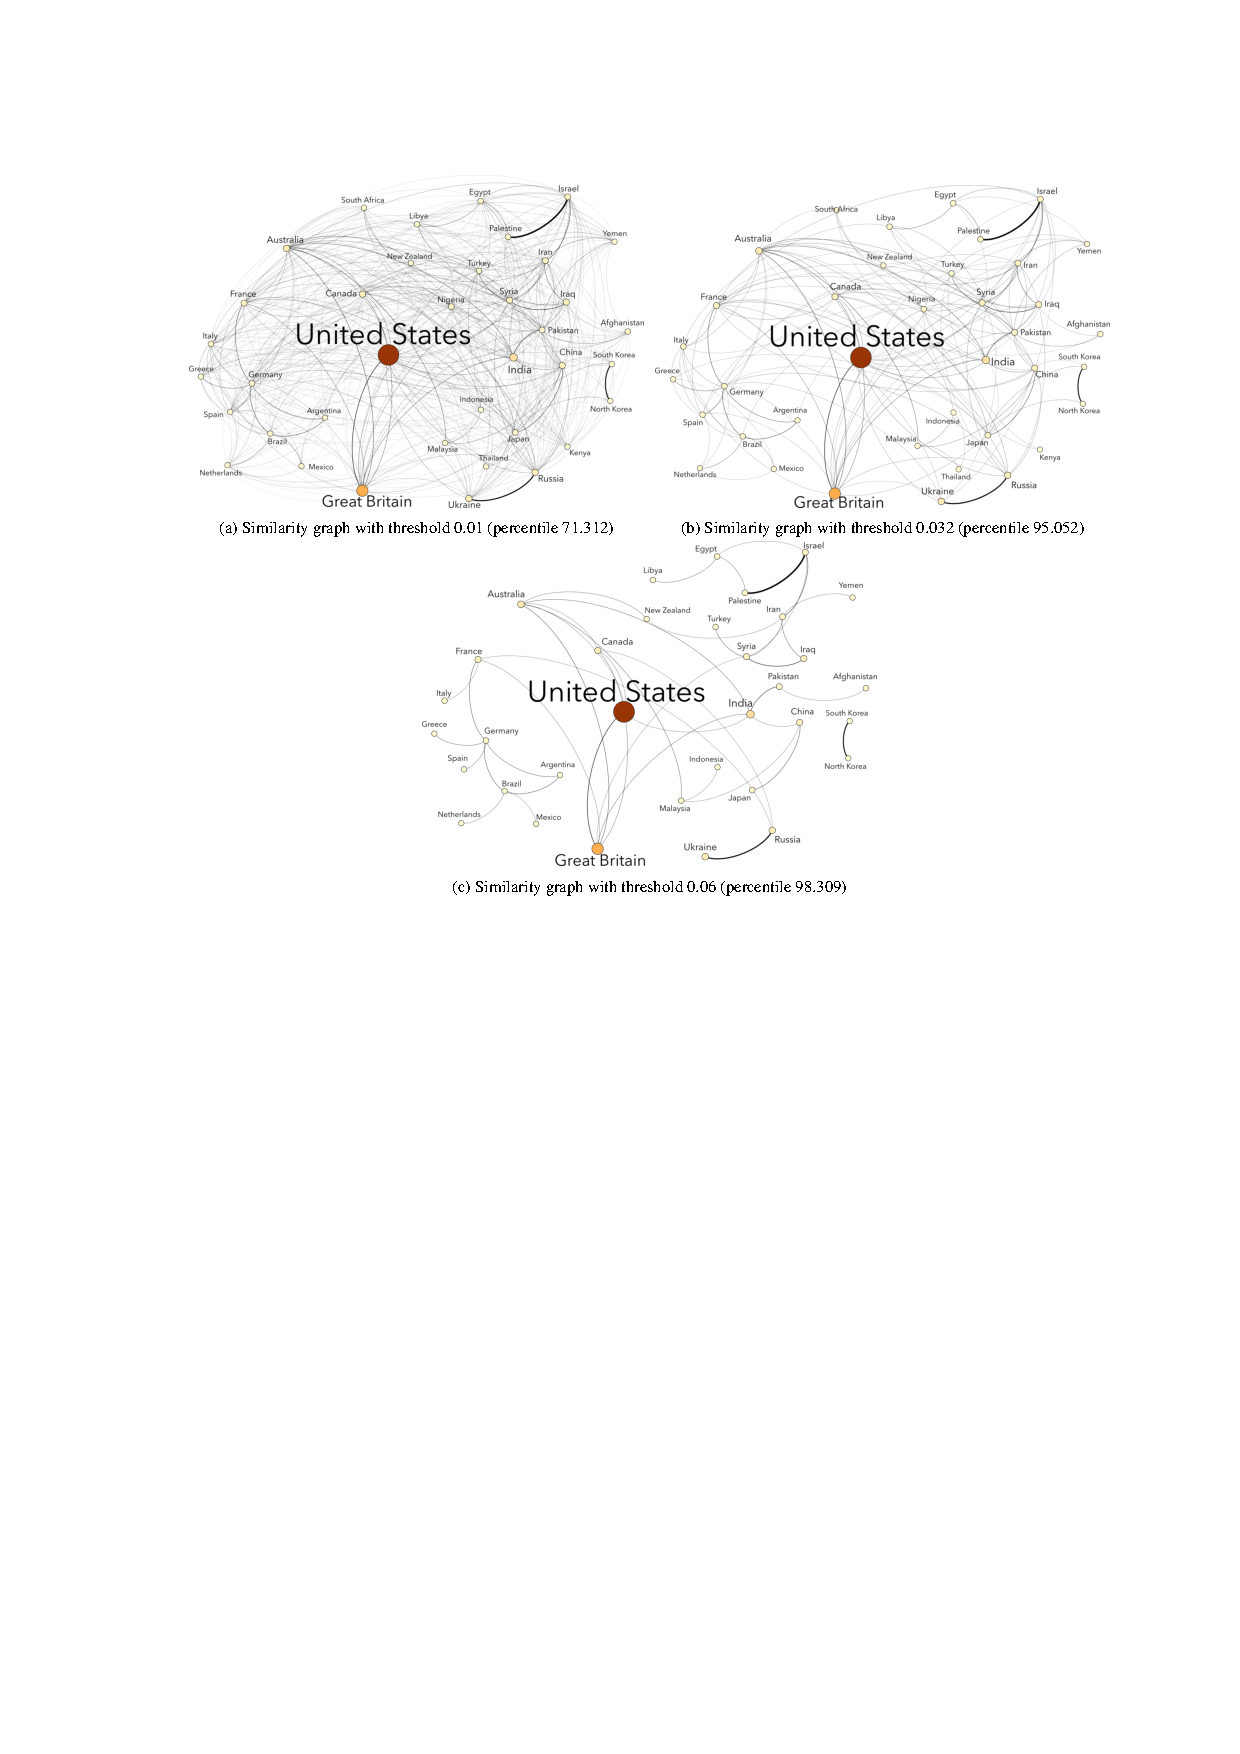
\includegraphics[width=1.15\textwidth]{figures/geopolitical/graphs.pdf}}%
    \caption[Graphs of similar countries]{Similarity graphs of countries using
    the Jaccard similarity as the weight for the edges. Each node is a country
    and an edge between two nodes corresponds to the Jaccard similarity between
    those two countries. An edge is present if the similarity is higher than the
    given threshold. The node size and color represents the number of events in
    which each country was a protagonist, and the thickness of and edge
    represents the similarity.}\label{fig:sim-graph}
\end{figure}

In Figure~\ref{fig:sim-graph}, we present three graphs where countries represent
nodes and edges are weighted based on the Jaccard similarity. 
%
As we increase the threshold to connect two countries with an edge, communities
of countries emerge. For example, in Figure~\ref{fig:sim-graph} (c), it is
possible to identify a group consisting of Germany, Mexico, Brazil, Argentina,
Netherlands, Spain and Italy: countries whose teams participated in the 2014
FIFA World Cup. 
%
It is also possible to observe edges among Malaysia, Indonesia, China and
Australia, reflecting the disappearance of the Malaysia Airlines flight MH370 on
2014. 
%
Those two long-term events, for instance, sparked several events in our dataset,
and the interactions between the protagonist countries are reflected in our
analysis.

\begin{figure}
    \centering
    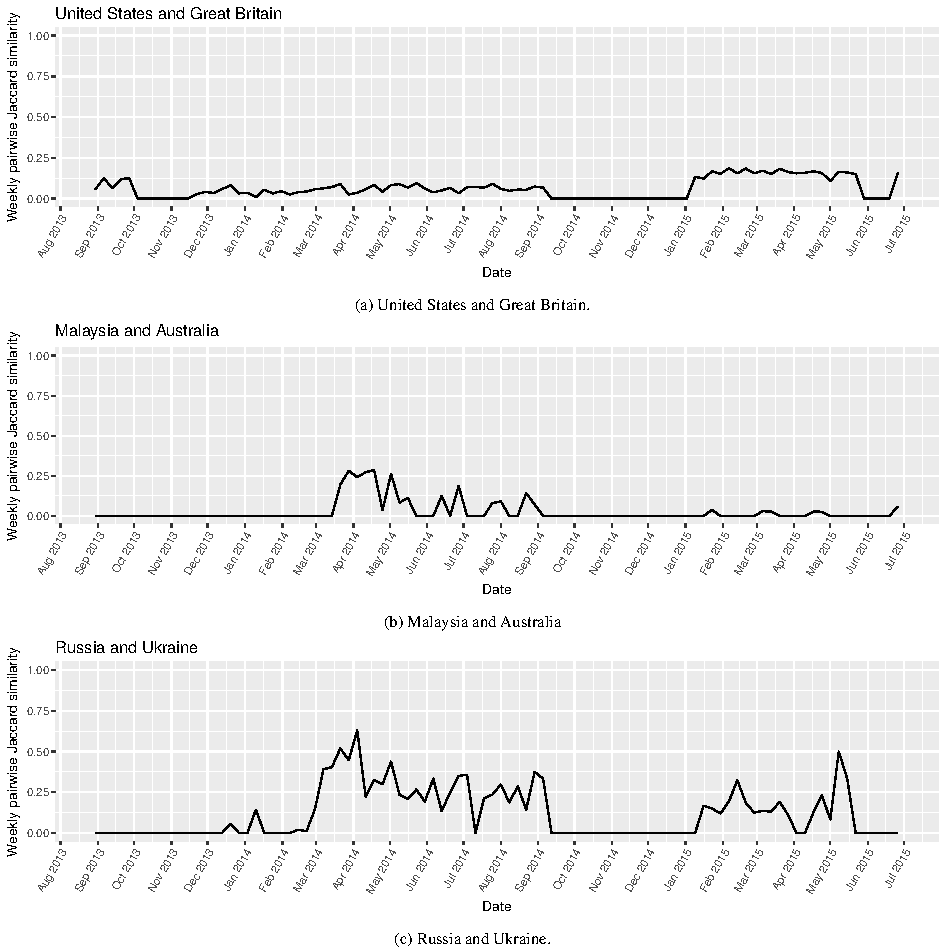
\includegraphics[width=\textwidth]{figures/geopolitical/jaccard_time.pdf}
    \caption[Time-series of the Jaccard similarity between co-protagonist
  vectors]{Time-series of the Jaccard similarity between co-protagonist vectors
  of selected pairs of countries over time. The value of similarity is computed
  for all the events in the given week. Data from October 2014 and December 2014
  was not available.}\label{fig:time-series}
\end{figure}

\paragraph{Time series of protagonist countries.}
We further explored trends of protagonist countries by analyzing the similarity
of countries over time. 
%
Given two countries, we computed their Jaccard similarity based on the events of
a time window of one week. 
%
Figure~\ref{fig:time-series} shows the time series between United States and
Great Britain, Malaysia and Australia, and Russia and Ukraine. 
%
Each of those pairs of countries showed different characteristics in terms of
how their similarity evolved over time. 
%
The US and Great Britain did not show notorious bursts of similarity over time,
although they had high overall Jaccard similarity (Table~\ref{tab:jacc}),
showing that although they were co-protagonists in several events, there was not
a particular situation that suddenly increased their similarity in a narrow time
span. 
%
On the other hand, Malaysia and Australia showed a burst starting in March 2014,
shortly after the disappearance of the Malaysia Airlines flight MH370 (similar
patterns arose when inspecting the relationship with Indonesia and China).
%
Finally, Russia and Ukraine showed high values of similarity over time, starting
roughly in December 2013 and those patterns were maintained throughout 2014.\\


% interest

Another aspect that we explored was the interest that different countries had in
events that occurred in different geographical regions. 
%
In other words, we explored the \emph{protagonist-interest} relationship between
countries. 
%
To do this, we represented each country $c_i$ as its corresponding
$\mathbf{pi}(c_i)$ vector (Equation~\ref{eq:pi}).


\begin{figure*}[t]
\centering
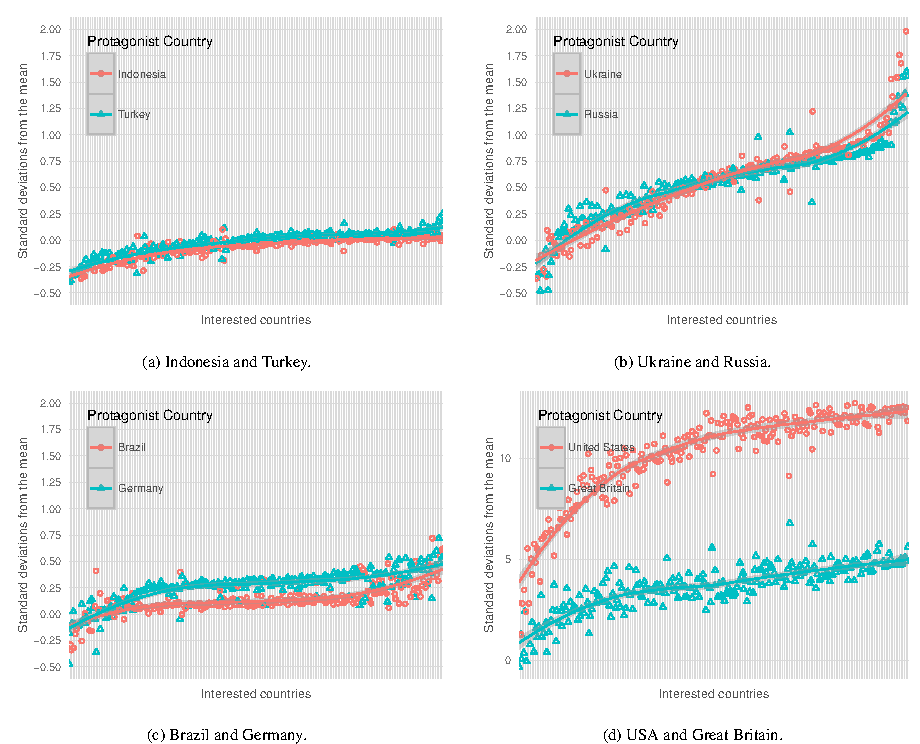
\includegraphics[width=\textwidth]{figures/geopolitical/int_prot.pdf}
\caption[Protagonist-interest plots for selected
countries.]{Protagonist-interest plots for selected countries.  Each plot shows
the level of interest ($y$-axis) displayed by the other counties of the world
(listed along the $x$-axis) in the events of the featured pair of ``protagonist
countries''. Country labels in the $x$-axis have been omitted for readability
purposes.}
\label{fig:int-prot}
\end{figure*}

We adjusted the original representation of the protagonist-interest vectors
(Equation~\ref{eq:pi}) in order to mitigate the data bias, which was reflected
in that some countries were overly represented, because they produced much more
tweets than others (Figure~\ref{fig:tweets-per} (a)). 
%
Then, instead of counting the number of events with $c_j$ as a protagonist, for
which $c_i$ expressed interest, we preferred to measure the interest of $c_i$ in
$c_j$ as the difference between the average number of events of other countries
in which $c_i$ was interested, with respect to the number of events of $c_j$ in
which $c_i$ was interested. 
%
In other words, our original interest measure was normalized by the average
interest shown by $c_i$ in other countries. 
%
Using this new interest measure we applied Euclidean distance to find the
country $c_2$ with the closest $\mathbf{pi}$ vector to another country $c_1$
(Table~\ref{tab:euc}).
%
Given that there were countries that expressed interest in only a few events, or
that were protagonists themselves of very few events, we only report the
countries that were protagonists of at least 167 events (i.e., the average
number of protagonist events per country in our dataset).

%%

We observed that Turkey had strong ties with other countries, being very close
with several other countries according to protagonist-interest relations, such
as Indonesia, Yemen, Afghanistan, Libya, and Malaysia. 
%
Furthermore, other similar countries were Italy and Japan, Brazil and Spain (and
also Brazil and Germany); these similarities are be explained by the events
triggered in the 2014 FIFA World Cup.
%
Notably, Russia and Ukraine standout again, showing not only that they were
protagonists of roughly the same events, but also that they were seen with
similar interest by the rest of the world, making the impact that the Ukrainian
crisis had on the news more evident.
%
We also noted that most of these countries are close geographically, and as well
as other countries, mostly from Asia.
%
We argue that these results are another sign of the bias in our dataset: the
perspective of international news as seen by English-speaking countries.

\begin{table}[t]
\centering
{\footnotesize
\begin{tabularx}{\textwidth}{@{}lrrrr@{}}
\toprule
Event Description & Tweets & Users & Outlets & Countries\\
\midrule
Death of actor Robin Williams (2014) & 1.8M & 1.3M & 48 & 202\\
FIFA World Cup final between Germany and Argentina (2014)  & 494K & 385K & 40 & 144\\
FIFA World Cup starts (2014)  & 476K & 358K & 45 &  143\\
Super Bowl starts (2015)  & 1.1M & 849K & 35 & 130\\
New Year's Eve (2013)  & 325K & 279K & 31 & 127\\
Soccer Player Luis Suarez is suspended from World Cup (2014)  & 213K & 157K & 38 & 106\\
Charlie Hebdo shooting in Paris (2015)  & 629K & 328K & 50 & 102\\
Grammy Awards (2015)  & 682K & 432K & 31 & 97\\
Boxing match between Mayweather and Pacquiao (2015)  & 779K & 522K & 37 & 97\\
\bottomrule
\end{tabularx}
}
\caption[Events with most international impact]{Events with most international impact, measured as the number of countries which showed interest higher than the 99-th percentile of overall interest.}\label{tab:impact}
\end{table}


% Please add the following required packages to your document preamble:
% \usepackage{booktabs}
\begin{table}
\centering
{\footnotesize
\begin{tabularx}{\textwidth}{@{}lrrr@{}}
\toprule
Event Description                                                 & Tweets & Distinct Users & Outlets \\ \midrule
US Supreme Court ruled in favor of same-sex marriage              & 51K  & 50K          & 7                                    \\
Delhi Legislative Assembly election                               & 35K  & 13K          & 3                                  \\
Labour party said it will scrap the non-domiciled tax status      & 32K  & 15K          & 10                           \\
Tornado strikes Texas                                             & 31K  & 6K           & 4                                    \\
TV appearance of Delhi chief minister candidate Arvind Kejriwal   & 30K  & 10K          & 1                                    \\
Hillary Clinton announces presidential bid                        & 30K  & 30K          & 3                                     \\
Football player Cardale Jones announces he is returning to school & 28K  & 22K          & 3                                      \\ \bottomrule
\end{tabularx}
}
\caption[Events with most local impact]{Events with most local impact, measured as the number of tweets coming from events with only one interested country, whose interest is higher than the 99-th percentile of overall interest. All events happened on 2015.}\label{tab:impact_local}
\end{table}



Finally, we explored events with the highest impact, considering international
and local events.  
%
For this analysis, we considered all international events (regional and global).
%
We counted the number of different interested locations for each event, however
only considering interest measurements within the 99-th percentile of the
dataset.
%
From this analysis we were able to observe that the events with the highest
overall impact covered several topics, and that the most recurrent events were
sports and entertainment.  
%
Events like the death of the actor Robin Williams caused the most international
impact, with a large number of tweets from 202 countries.  
%
This was followed by sports events, such as the 2014 FIFA World Cup, the 2013
Super Bowl and the boxing match between Floyd Mayweather and Manny Pacquiao
(Table~\ref{tab:impact}).
%
Other events with high impact included New Year's Eve for 2013, the
\emph{Charlie Hebdo} shooting in Paris, and the Grammy Awards in 2015.  
%
We also observed that the coverage of different news outlets was higher for
these events.
%
On the other hand, events with local impact consisted mostly of political
events, such as political elections and debates, with the exception of a natural
disaster and a sports event.
%
We observed that in this case the coverage of different news sources was lower
in relation to high impact international events, as well as the number of tweets
involved.

%%

The source code of the analysis above and more examples can be found in the
following URL: \url{https://users.dcc.uchile.cl/~mquezada/galean/analysis.html}
(Accessed: June 21, 2019).